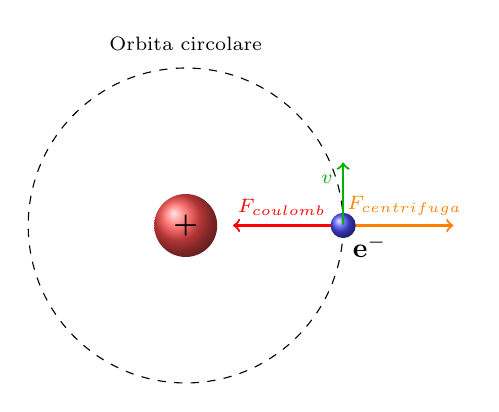
\begin{tikzpicture}[scale=2]
    % Nucleo
    \shade[ball color=red!70] (0,0) circle (0.2);
    \node at (0,0) {\textbf{+}}; % carica positiva
    
    % Orbita
    \draw[thin, dashed] (0,0) circle (1.0);
    \node[above] at (0,1.05) {\scriptsize Orbita circolare};
    
    % Elettrone
    \shade[ball color=blue!70] (1.0,0) circle (0.08);
    \node[below right] at (1.0,0) {\textbf{e$^-$}};
    
    % Forza coulombiana (verso il nucleo)
    \draw[->, thick, red] (0.92,0) -- (0.3,0)
        node[midway, above] {\scriptsize $F_{\text{coulomb}}$};
    
    % Forza centrifuga (verso l'esterno)
    \draw[->, thick, orange] (1.08,0) -- (1.7,0)
        node[midway, above] {\scriptsize $F_{\text{centrifuga}}$};
    
    % Velocità tangenziale
    \draw[->, thick, green!70!black] (1.0,0) -- (1.0,0.4)
        node[midway, above left] {\scriptsize $v$};
\end{tikzpicture}
